\chapter{Planar flows}
\label{ch:planflow}

\section{Learning objectives}

At the end of this lesson, a student should be able to
\begin{enumerate}
\item pick a combination of elementary planar flows that suit a given flow condition
\item plot contours of stream function and interpret the direction of the flow field at a given location
\end{enumerate}

\section{Reducing the number of unkown velocity components}

{\bf Continuity equation of an incompressible fluid}
Rectangular coordinate sytem:
$$ \vec{\nabla} \cdot \vec{u} = {\partial u_1 \over \partial x_1} + {\partial u_2 \over \partial x_2} + {\partial u_3 \over \partial x_3} = 0  $$
Cylindrical coordinates:
$$ \vec{\nabla} \cdot \vec{V} = {1 \over r} {\partial \over \partial r} \left( r V_r \right) + {1 \over r} {\partial V_\theta \over \partial \theta} + {\partial V_z \over \partial z} = 0 $$
Spherical coordinates:
$$ \vec{\nabla} \cdot \vec{V} = {1 \over r^2} {\partial \over \partial r} \left( r^2 V_r \right) + {1 \over r \sin\theta} {\partial \over \partial \theta} \left( V_\theta \sin\theta \right) + {1 \over r \sin\theta} {\partial V_\phi \over \partial \phi} = 0 $$
\begin{enumerate}
\item Validate components of a velocity field
\item Determine a velocity components if rest are known
\item For 2D flows, reduce the velocity field to a scalar function
\end{enumerate}

% -----------------------------------------------------------------------

{\bf Planar flow concepts}
Concepts to be familiar with:
\begin{enumerate}
\item Stream function $\psi$
\item Potential $\Phi$
\item Vorticity $\omega$
\end{enumerate}

Elementary planar flows: 
\begin{enumerate}
\item Uniform flow
\item Source flow
\item Sink flow
\item Doublet
\item Vortex
\end{enumerate}

% -----------------------------------------------------------------------

% learning objective
\begin {lo3} [Fluid Flow]
Apply definition of stream function to determine velocity components
\end {lo3}

\section{Stream function}

\index{Stream function}

Convince yourself that the following definitions of the velocity components from their respective stream function $\psi$ will satisfy the continuity equation for {\bf any} continuous and well behaved scalar function $\psi$.

Definition of stream function $\psi$ in rectangular coordinate system is given as follows so that $\vec{\nabla} \cdot \vec{u} = 0$ for a 2D flow:

$$ u_x \equiv {\partial \psi \over \partial y} \hspace{1 in} u_y \equiv -{\partial \psi \over \partial x}$$

Definition of stream function $\psi$ in cylindrical coordinate system is given as follows.

$$ v_r \equiv {1 \over r}{\partial \psi \over \partial \theta} \hspace{1 in} v_\theta \equiv -{\partial \psi \over \partial r}$$

Irrotational flow is one in which fluid elements moving in the flow field do not undergo any rotation. This is expected when viscous forces are not dominant. This needs the condition $\vec{\nabla} \times \vec{u} =0$. Such a flow field can be represented using a potential $\phi$ defined as follows.
$$ \vec{u} = -\vec{\nabla} \phi$$

Velocity components for a potential flow in rectangular coordinate system are given as follows.

$$ u_x = -{\partial \phi \over \partial x} \hspace{1 in} u_y = -{\partial \phi \over \partial y}$$

Velocity components for a potential flow in cylindrical coordinate system are given as follows.

$$ u_r = -{\partial \phi \over \partial r} \hspace{1 in} u_\theta = -{1 \over r}{\partial \phi \over \partial \theta}$$


\subsection{Rectangular}

Continuity equation in rectangular coordinates:

$$\vec{\nabla} \cdot \vec{V} = {\partial V_x \over \partial x} + {\partial V_y \over \partial y} + {\partial V_z \over \partial z} = 0$$

Case 1: $V_z = 0$, No $z$-dependence

$$V_x = {\partial \psi \over \partial y} $$

$$V_y = - {\partial \psi \over \partial x} $$

Following relation comes from these definitions easily.

$$ {\partial V_x \over \partial y} - {\partial V_y \over \partial x} = \nabla^2 \psi$$

\subsection{Cylindrical}

Continuity equation in Cylindrical coordinates:

$$ \vec{\nabla} \cdot \vec{V} = {1 \over r} {\partial \over \partial r} \left( r V_r \right) + {1 \over r} {\partial V_\theta \over \partial \theta} + {\partial V_z \over \partial z} = 0 $$

Case 2: $V_z = 0$, No $z$-dependence:
 $$ V_r = {1 \over r} {\partial \psi \over \partial \theta} $$
 $$ V_\theta = - {\partial \psi \over \partial r} $$


Case 3: $V_\theta = 0$, No $\theta$-dependence:
 $$ V_r = {1 \over r} {\partial \psi \over \partial z} $$
 $$ V_z = -{1 \over r} {\partial \psi \over \partial r} $$



\subsection{Spherical}

Continuity equation in Spherical coordinates:

$$ \vec{\nabla} \cdot \vec{V} = {1 \over r^2} {\partial \over \partial r} \left( r^2 V_r \right) + {1 \over r \sin\theta} {\partial \over \partial \theta} \left( V_\theta \sin\theta \right) + {1 \over r \sin\theta} {\partial V_\phi \over \partial \phi} = 0 $$

Case 4: $V_\phi = 0$, No $\phi$-dependence:
 $$ V_r = {1 \over r^2 \sin\theta} {\partial \psi \over \partial \theta} $$
 $$ V_\theta = - {1 \over r \sin\theta} {\partial \psi \over \partial r} $$

\begin{quote}
{\bf Classwork:} Convince yourself that the above components of the velocity in 2D flow satisfy the corresponding form of continuity equation.
\end{quote}


Stream function is represented as $\psi\left(x,y\right)$ in a 2D rectangular coordinate system.

Assume $V_z = 0$, no $z$-dependence of other components

Continuity equation in 2D:
$${\partial V_x \over \partial x} + {\partial V_y \over \partial y} = 0$$

Define $\psi$ such that:

$$V_x = {\partial \psi \over \partial y} \, \& \, V_y = - {\partial \psi \over \partial x} $$
Continuity equation is satisfied for {\bf any well behaved} $\psi\left(x,y\right)$


% -----------------------------------------------------

{\bf Sign convention relating $\psi$ and velocity}


\begin{figure}[h]
\begin{center}
\framebox{ 
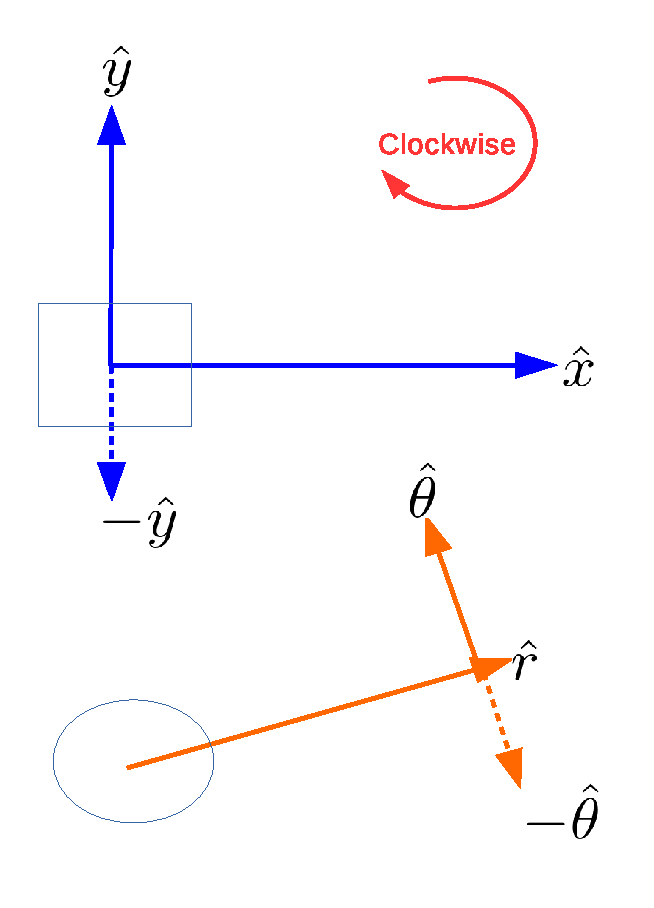
\includegraphics[scale=0.5]{images/c08-psisignconvention.eps}
}
\end{center}
\caption{Sign convention for stream function}
\label{psisignconvention}
\end{figure}


    Rectangular: 
    $$V_x = {\partial \psi \over \partial y} \, \& \, V_y = - {\partial \psi \over \partial x} $$
{\bf Convention}
Differentiation of $\psi$ in a direction gives velocity component $90^o$ clockwise from that direction.
    Cylindrical:
 $$ V_r = {1 \over r} {\partial \psi \over \partial \theta} \, \, \& \, \, V_\theta = - {\partial \psi \over \partial r} $$

{\bf Meaning of $\psi$}


\begin{figure}[h]
\begin{center}
\framebox{ 
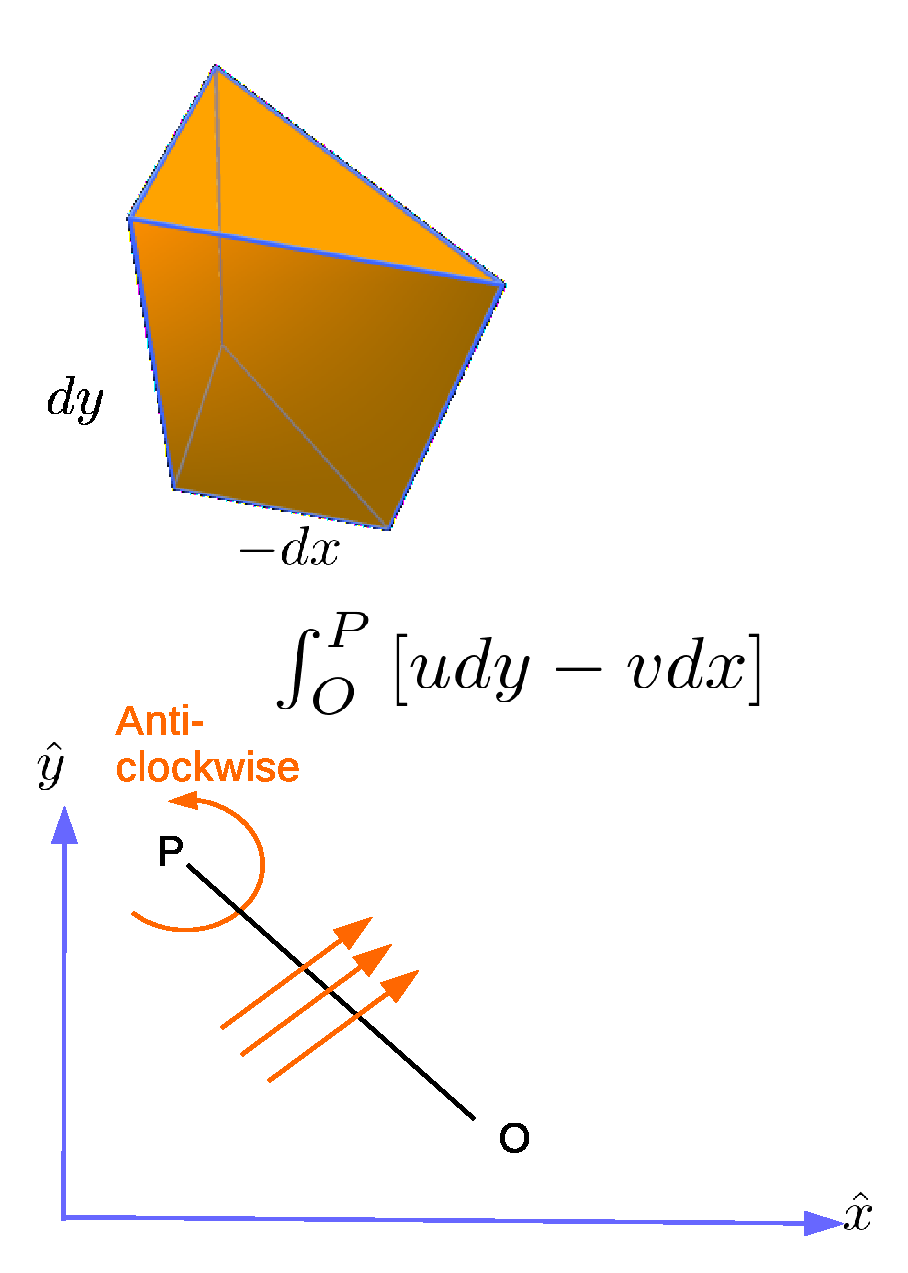
\includegraphics[scale=0.5]{images/c08-psiflowconvention.eps}
}
\end{center}
\caption{Convention for flow direction using contours of stream function}
\label{psiflowconvention}
\end{figure}

If the flow is two dimensional, with only $r$ and $\theta$ components, then we can introduce the stream function $\psi$ as 

\begin{equation}
u_r \equiv {1 \over r} {\partial \psi \over \partial \theta}
\end{equation}

\begin{equation}
u_\theta \equiv - {\partial \psi \over \partial r}
\end{equation}

such that the continuity equation 

\begin{equation}
{\partial \left(r u_r\right) \over \partial r} + {\partial u_\theta \over \partial \theta} = 0
\end{equation}

is satisfied by the fact that the order of differentiation of $\psi$ with respect to $r$ and $\theta$ does not matter.


{\bf Convention}
Flux of fluid volume across a line OP is taken positive when it is in the anti-clockwise sense about P.

Exact differential of $\psi$:
$$ d\psi = {\partial \psi \over \partial x} dx +  {\partial \psi \over \partial y} dy = -v dx + u dy $$
$$ \psi_P - \psi_O = \int_{O}^{P}{\left[u dy - v dx\right]}$$

$\psi$ is flux of fluid volume across a line OP.

% -----------------------------------------------------

{\bf Stream function $\psi\left(r,\theta\right)$}

Assume $V_z = 0$, no $z$-dependence

Continuity equation in 2D:
$$ {1 \over r} {\partial \over \partial r} \left( r V_r \right) + {1 \over r} {\partial V_\theta \over \partial \theta} = 0 $$

Define $\psi$ such that:
 $$ V_r = {1 \over r} {\partial \psi \over \partial \theta} \, \, \& \, \, V_\theta = - {\partial \psi \over \partial r} $$


% -----------------------------------------------------

{\bf Stream function $\psi\left(r,z\right)$}

Assume $V_\theta = 0$, no $\theta$-dependence

Continuity equation in 2D:
$$ {1 \over r} {\partial \over \partial r} \left( r V_r \right) + {\partial V_z \over \partial z} = 0 $$

Define $\psi$ such that:
 $$ V_r = {1 \over r} {\partial \psi \over \partial z} \, \, \& \, \, V_z = -{1 \over r} {\partial \psi \over \partial r} $$

% -----------------------------------------------------

{\bf Stream function $\psi\left(r,\theta\right)$}

Assume $V_\phi = 0$, no $\phi$-dependence

Continuity equation in 2D:
$$ {1 \over r^2} {\partial \over \partial r} \left( r^2 V_r \right) + {1 \over r \sin\theta} {\partial \over \partial \theta} \left( V_\theta \sin\theta \right) = 0 $$

Define $\psi$ such that:
 $$ V_r = {1 \over r^2 \sin\theta} {\partial \psi \over \partial \theta} \, \, \& \, \, V_\theta = - {1 \over r \sin\theta} {\partial \psi \over \partial r} $$


% -----------------------------------------------------------------------

% learning objective
\begin {lo3} [Fluid Flow]
Validate a velocity profile as irrotational
\end {lo3}

\section{Vorticity}

Vorticity is often represented using $\omega$.

{\bf Definition}
$$ \omega = \vec{\nabla} \times \vec{u}$$

{\bf Circulation} $\Gamma$ is line integral of tangential velocity component about a closed curve C fixed in the flow.
$$ \Gamma = \oint_{C}{\vec{u} \times \vec{dS}}$$

Stokes theorem in 2D:
$$ \Gamma = \oint_{C}{\vec{u} \times \vec{dS}} = \int_{A}{\vec{\nabla} \times \vec{u} dA} =  \int_{A}{\vec{\omega} \cdot \hat{n} dA} $$ 

In an {\bf irrotational} flow fluid elements do not undergo any rotation:
$$ \omega = 0 $$ 

% -----------------------------------------------------------------------

% learning objective
\begin {lo3} [Fluid Flow]
Apply definition of velocity potential to determine velocity components
\end {lo3}

\section{Velocity potential}

Velocity potential is often represented using $\Phi$.

Using the vector identity $\vec{\nabla} \times \vec{\nabla} \Phi = 0$ for any scalar function $\Phi$, one can propose a {\bf potential} to determine velocity fields of an {\bf irrotational flow}.

Flow is down the potential gradient. Let's define $\Phi$ such that:
$$ \vec{u} = -\vec{\nabla}\Phi $$
$$ u_1 = -{\partial \Phi \over \partial x_1} \, \, \& \, \, u_2 = -{\partial \Phi \over \partial x_2} $$


% -----------------------------------------------------------------------

{\bf Generating velocity potentials}

Continuity equation for incompressible fluids:
$$ \vec{\nabla} \cdot \vec{u} = - \vec{\nabla} \cdot \vec{\nabla}\Phi = 0 \implies  \nabla^2 \phi = 0 $$

Any scalar function that satisfies the Laplace's equation can be used as $\Phi$ to generate 2D velocity field.

Unlike stream function, velocity potentials can be used in 3D too.


% -----------------------------------------------------------------------

\section{Potential flow}

Potential flow in cylindrical coordinate system:

Define $\Phi$ such that:
$$ u_r = -{\partial \Phi \over \partial r} \, \, \& \, \, u_\theta = -{1 \over r}{\partial \Phi \over \partial \theta} $$

Continuity equation in 2D becomes:
$$ {\partial^2 \Phi \over \partial r^2} + {1 \over r}{\partial \Phi \over \partial r}+ {1 \over r^2} {\partial^2 \Phi \over \partial \theta^2} = -\nabla^2 \Phi = 0 $$

Any scalar function that satisfies the Laplace's equation can be used as $\Phi$ to generate 2D velocity field.

% -----------------------------------------------------------------------

{\bf Stream function and velocity potential}

\begin{enumerate}
\item Difference in values of contours of $\psi$ represent volume flow between them.
\item Velocity vector at any point is tangential to the contour of $\psi$ through the point
\item Contours of $\psi$ indicate the sense of flow.
\item Contours of $\Phi$ are normal to those of $\psi$.
\end{enumerate}


% -----------------------------------------------------------------------

% learning objective
\begin {lo3} [Fluid Flow]
Plot elementary planar flows
\end {lo3}

\section{Elementary planar flows}

\subsection{Uniform flow}

Stream function $\psi$:

$\psi = A y$ or $\psi = Ar \cos\theta$

Velocity Potential $\Phi$:

$\Phi = -A x$ or $\Phi = Ar \sin\theta$

Velocities:

$ u = A$, $v=0$

\begin{figure}[h]
\begin{center}
\framebox{ 
\includegraphics[scale=0.5]{images/c08-UniformFlow.ps}
}
\end{center}
\caption{Uniform flow using potential function}
\label{planaruniformflow}
\end{figure}



% -----------------------------------------------------------------------

\subsection{Stagnation flow}

Stream function $\psi$:

$$\psi = -2xy$$
Velocity Potential $\Phi$:
$$\Phi = x^2 - y^2$$
Velocities:

$ u = -2x$ \, $v = 2y$

\begin{figure}[h]
\begin{center}
\framebox{ 
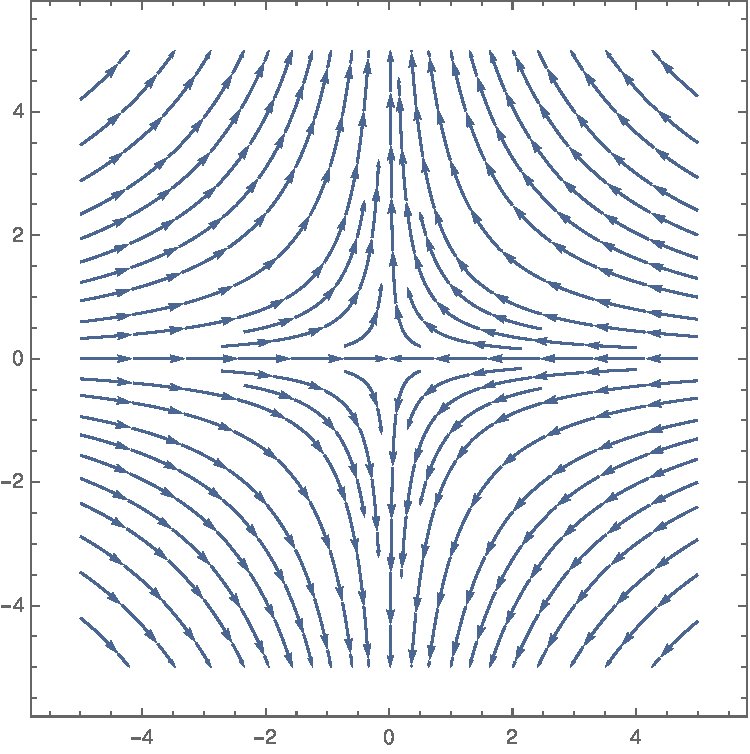
\includegraphics[scale=0.5]{images/c08-StagnationFlow.ps}
}
\end{center}
\caption{Stagnation flow using potential function}
\label{planarstagnationflow}
\end{figure}


% -----------------------------------------------------------------------

\subsection{Sink flow}

$Q$ is  volume flow rate per unit depth

Stream function $\psi$:

$\psi = {-Q \over 2\pi} \theta$

Velocity Potential $\Phi$:

$\Phi = {Q \over 2\pi} \ln r$

Velocities:

$u_r = {-Q \over 2 \pi r}$,  $u_\theta = 0$

\begin{figure}[h]
\begin{center}
\framebox{ 
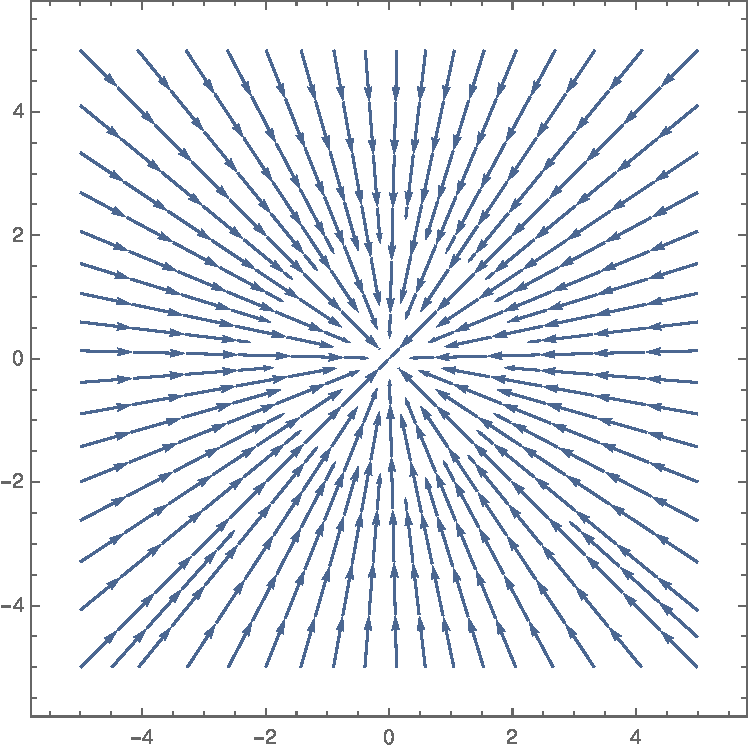
\includegraphics[scale=0.5]{images/c08-SinkFlow.ps}
}
\end{center}
\caption{Sink flow using potential function}
\label{planarsinkflow}
\end{figure}


% -----------------------------------------------------------------------
\subsection{Source flow}

$Q$ is  volume flow rate per unit depth

Stream function $\psi$:

$\psi = {Q \over 2\pi} \theta$

Velocity Potential $\Phi$:

$\Phi = {-Q \over 2\pi} \ln r$

Velocities:

$u_r = {Q \over 2\pi r}$,  $u_\theta = 0$

\begin{figure}[h]
\begin{center}
\framebox{ 
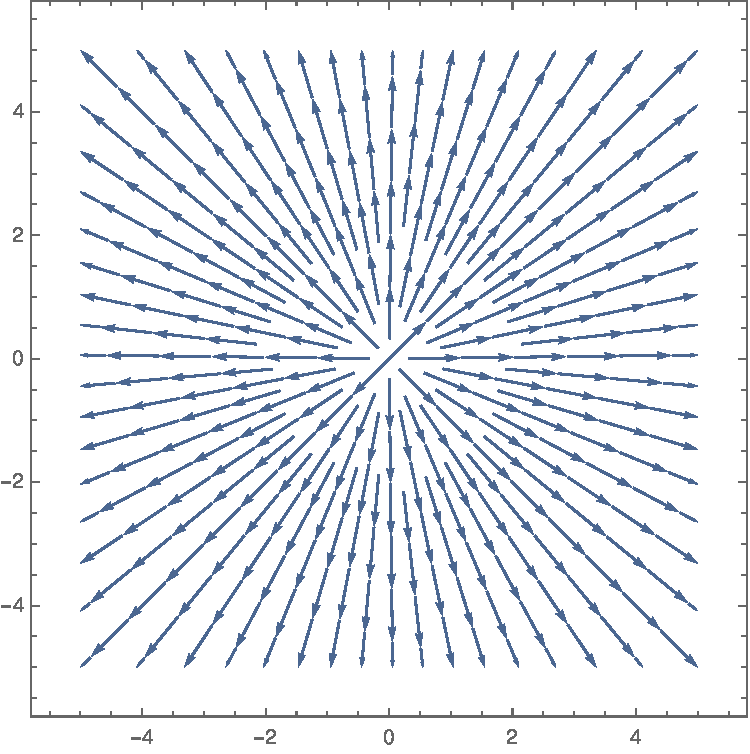
\includegraphics[scale=0.5]{images/c08-SourceFlow.ps}
}
\end{center}
\caption{Source flow using potential function}
\label{planarsourceflow}
\end{figure}

% -----------------------------------------------------------------------

\subsection{Doublet}

$A$ is strengh of doublet.

Stream function $\psi$:
$$\psi = {-A \sin\theta \over r}$$

Velocity Potential $\Phi$:
$$\Phi = {-A\cos\theta \over r}$$

Velocities:

$u_r = {-A \cos\theta \over r^2}$, $u_\theta = {-A \sin\theta \over r^2}$

\begin{figure}[h]
\begin{center}
\framebox{ 
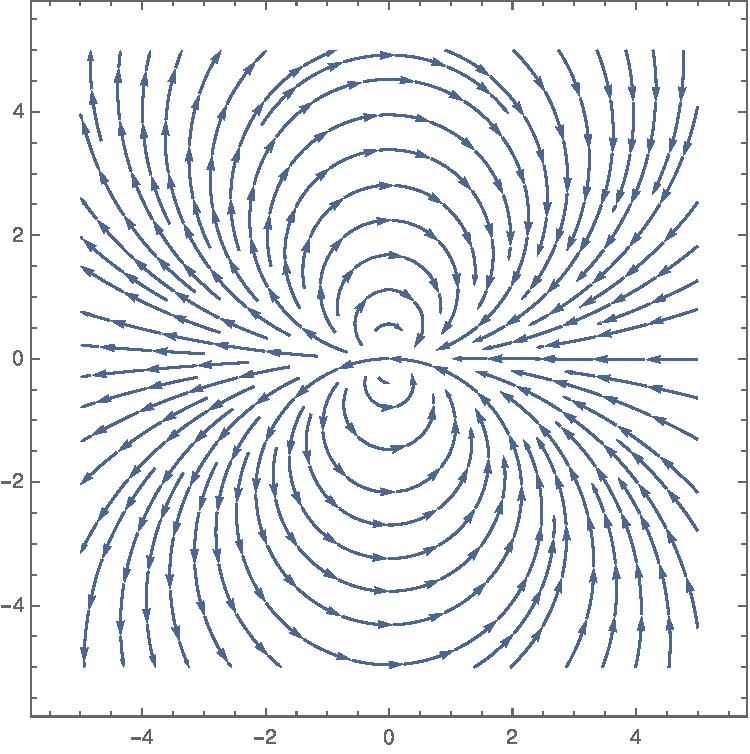
\includegraphics[scale=0.4]{images/c08-Doublet.ps}
}
\end{center}
\caption{Doublet flow using potential function}
\label{planardoubletflow}
\end{figure}


% -----------------------------------------------------------------------
\subsection{Vortex}

$A$ is strength of vortex

Stream function $\psi$:
$$\psi = {-A \over 2\pi} \ln r$$

Velocity Potential $\Phi$:

$$\Phi = {-A \over 2 \pi} \theta $$

Velocities:

$u_r =0$, $u_\theta={A \over 2 \pi r}$

\begin{figure}[h]
\begin{center}
\framebox{ 
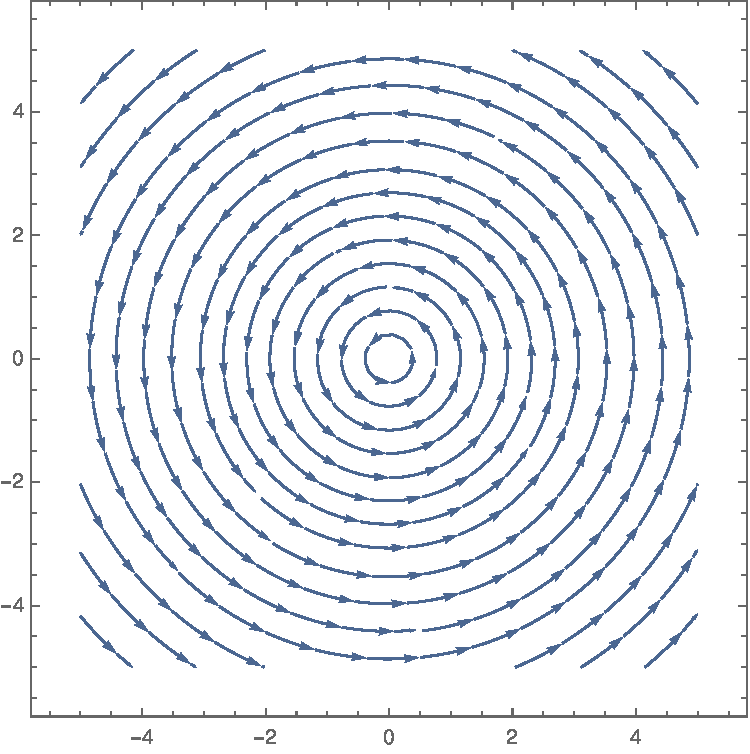
\includegraphics[scale=0.4]{images/c08-Vortex.ps}
}
\end{center}
\caption{Vortex flow using potential function}
\label{planarvortexflow}
\end{figure}


% -----------------------------------------------------------------------

\subsection{Combinations of elementary planar flows}

Source flow + Uniform flow $\rightarrow$ Flow past a half-body

\begin{figure}[h]
\begin{center}
\framebox{ 
\includegraphics[scale=0.4]{images/c08-SourceUniform.ps}
}
\end{center}
\caption{Source + Uniform flow using potential function}
\label{planarsourceuniformflow}
\end{figure}


Source or Sink flow + Vortex $\rightarrow$ Spiral flow
\begin{figure}[h]
\begin{center}
\framebox{ 
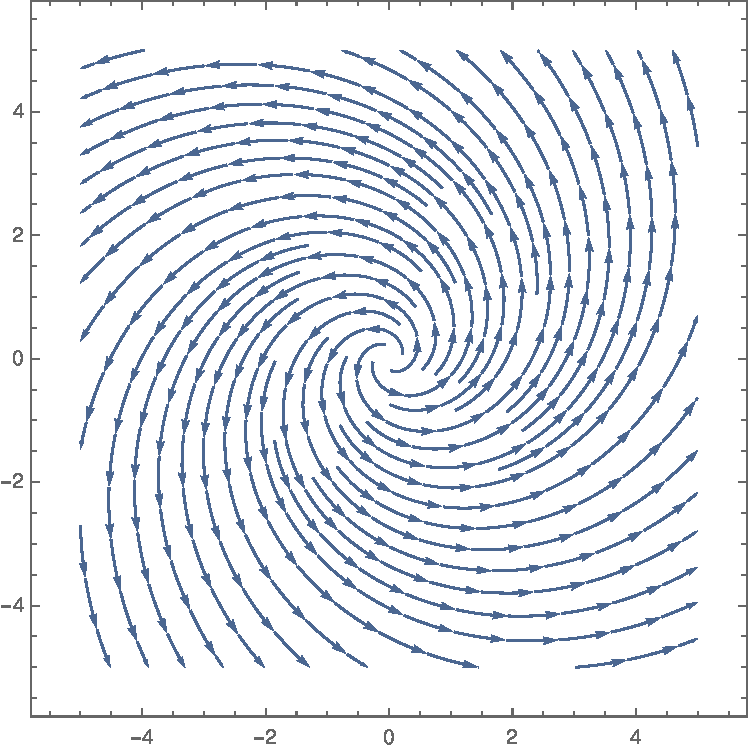
\includegraphics[scale=0.4]{images/c08-SourceVortex.ps}
}
\end{center}
\caption{Source + Vortex flow using potential function}
\label{planarsourcevortexflow}
\end{figure}


% -----------------------------------------------------------------------

{\bf Combinations of elementary planar flows}

Doublet + Uniform flow $\rightarrow$ Flow past a cylinder

\begin{figure}[h]
\begin{center}
\framebox{ 
\includegraphics[scale=0.4]{images/c08-DoubletUniform.ps}
}
\end{center}
\caption{Doublet + Uniform flow using potential function}
\label{planardoubletuniformflow}
\end{figure}


Doublet +Vortex + Uniform flow $\rightarrow$ Flow past a cylinder with circulation

\begin{figure}[h]
\begin{center}
\framebox{ 
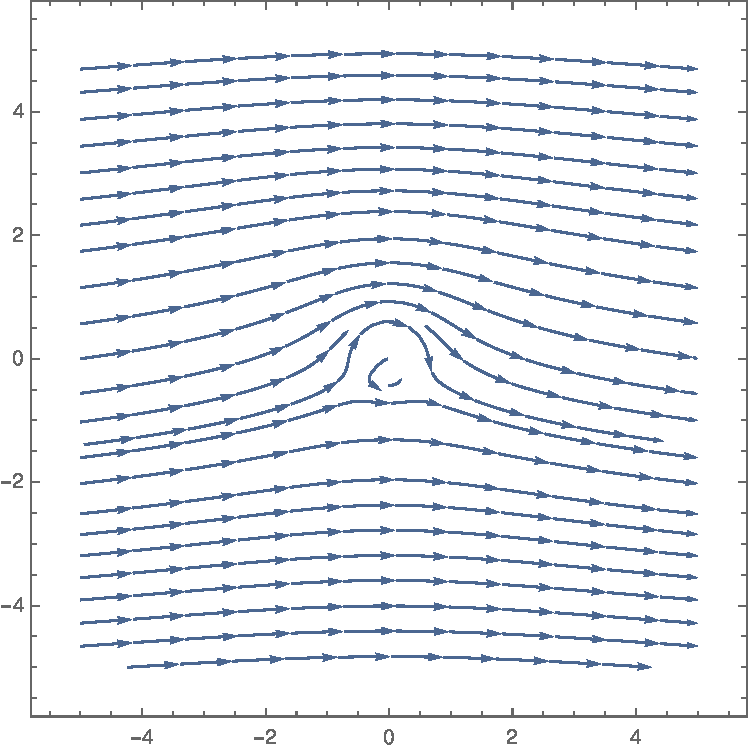
\includegraphics[scale=0.4]{images/c08-DoubletVortexUniform.ps}
}
\end{center}
\caption{Doublet + Vortex + Uniform flow using potential function}
\label{planardoubletvortexuniformflow}
\end{figure}


% -----------------------------------------------------------------------

%{\bf Applications in materials processing}
%Tapping liquid metal from a ladle
%\includegraphics[width=5in]{images/TundishMold.png}\\
%\includegraphics[width=5in]{images/concast.png}\\
%{\small ref: \tt www.wikipedia.com}

%Gas flow through nozzles
%\includegraphics[width=5in]{images/GTAW.jpg}\\
%{\small ref: \tt www.wikipedia.com}

% -----------------------------------------------------------------------

\section{Summary}

\begin{enumerate}
\item Stream function relations
\item Vorticity relations
\item Condition for irrotational flow
\end{enumerate}

% -----------------------------------------------------------------------

\section{Further study}

\begin{enumerate}
\item The velocity field near the core of a tornado can be approximated as following.
$$ \vec{u} = -{q \over 2 \pi r} \hat{e}_r + {K \over 2 \pi r} \hat{e}_\theta $$
Is this an irrotational flow field? Obtain the stream function for this flow. \\ Ans: $\psi = -\left( q\theta+K\ln r \right)/2\pi$.

\item An incompressible flow field is defined using stream function as follows. $$ \psi = A\left(x^2-y^2\right)$$
Determine the velocity components of this flow field. Also, check if this flow field is irrotation and if so, determine the velocity potential $\phi$ for this flow.

\item Using the definitions of $\psi$ and $\phi$ and the continuity equation for a 2D flow field, show that any scalar function that satisfies the Laplace's equation can represent a 2D, irrotational, incompressible flow field.

\item Volume flow rate across two streamlines is given by $Q=\int{u dl}$ where $l$ is the distance across the two streamlines. Convince yourself that the volume flow rate Q between two streamlines $\psi_1$ and $\psi_2$ is $\psi_2-\psi_1$. \\ Hint: Write the exact differential for $\psi$ and evaluate the flow rate between two streamlines keeping either $x$ or $y$ constant.

\item Convince yourself that the constant $\psi$ line at any point is negative reciprocal to the slope of $\phi$ at that point.\\ Hint: Use exact differential of $\psi$ and $\phi$ and write $ \left( {\partial y \over \partial x} \right)_\psi$ etc.,

\item A flow field where the streamlines are concentric circles is called a vortex. What kind of functional form can you think of for the velocity components in a vortex?
 
\item During welding, argon gas jet is used to protect the liquid melt pool. The gas flows down the cylindrical tube kept at a small height from the plate being welded. Draw schematically the flow field for this situation and design a possible functional form for the velocity components in different regions of this problem.\\ Hint: There are regions where the flow is unidirectional and where the flow is radially outward (source flow). 

\end{enumerate}

% -----------------------------------------------------------------------
